The motion of a golf ball can fundamentally be viewed as a set of forces acting on the ball as it
flies through the air. Before we can obtain a better understanding of the nature of the drag and lift,
or characterise a ball by the lift and drag functions we find,
obtaining a model for the forces acting on the ball during the flight is advisable. 

Here, we follow the paper by \citet{Robinson2013}, which builds a model of the flight based on simple principles as
we desire. This model does neglect some of the subtlety of the fluid dynamics we have discussed,
but is a useful starting point for the analysis.

\section{A Model for Golf Ball Flight}

In \citet{Robinson2013} the authors first discuss the assumptions and limitations of the model at hand.
We will take the reverse to this approach, discussing the features of the model and then mentioning
some of the potential improvements to the model and the drag and lift form they give.

Additionally, the authors give a sample MATLAB script for the setup of the differential equations they
derive and suggest using MATLAB to solve the resultant differential equations of the model numerically. 
This sample code forms the bases of our initial investigations into the trajectories.

\subsection{Lift and Drag}

\citeauthor*{Robinson2013} start by initially discussing the lift and drag forces on a golf ball.
They use the form of the lift and drag in the high Reynolds number limit, given by

\begin{equation} \nonumber
F_{D} = \frac{1}{2} \rho \vv^2 A c_{D}
\end{equation}
and
\begin{equation} \nonumber
F_{L} = \frac{1}{2} \rho \vv^2 A c_{L}
\end{equation}

The use of this form of equation is justified by the authors stating that there is experimental evidence
that golf ball flight always occurs at $Re > 10^3$. We will examine this assumption later.

\subsubsection{Drag}

The authors give a form for $c_D$ based on the spin of the ball
\begin{equation}
c_D = 0.3 + 2.58\times10^{-4}\omega
\end{equation}
where $\omega$ is the modulus of $\vec{\omega}$ the spin vector, in radians per second. This is obtained 
from experimental results found by
\citet{davies1949aerodynamics}. However, the authors elect to take $c_D = 0.45$, rationalising that
this simplification is most suited to the range of spins and speeds which golf balls are likely to
take. The authors also mention the lack of experimental evidence they found to suggest better forms
for $c_D$.

\subsubsection{Lift}

\citeauthor*{Robinson2013} make the following assumptions for the lift on the golf ball:
\begin{itemize}
\item The direction of the lift for is perpendicular to both $\omega$ and $\vv$, that is $\vec{F}_{L} \propto \omega \times \vv$.
\item The lift is not a function of the drag.
\end{itemize}

They then go on to express the lift force as a vector quantity, given by
\begin{equation}
\vec{F}_{L} = \frac{1}{2} \rho A c_{L} V^2 \sin \theta \cdot \hat{n}
\end{equation}
and then using the definition of cross products rewrite this as
\begin{equation}
\vec{F}_L = \frac{1}{2} \rho A c_L V \cdot \left(\frac{\vec{\omega} \times \vv}{\omega}\right)
\end{equation}
which is the form used in the model.

As with $c_D$, the authors then use experimental data to inform their choice for $c_L$, once again
following \citet{davies1949aerodynamics} to find that
\begin{equation} \label{cl-rr}
c_L = 3.19\times10^{-1} \left(1 - \exp(-2.48\times10^{-3} \omega)\right)
\end{equation}
fits with a number of different experimental studies of the lift over spheres.

The authors also state that this form completely omits any possibility of a negative Magnus effect 
pushing the ball towards the ground.

\subsection{Accounting for the Wind}

In order to deal with the effect of the wind on the golf ball the authors introduce a new $\vec{v}$
which is defined as being the velocity of the ball relative to the air. That is, if the wind is blowing
with a velocity $\vec{W}$ and the ball moving with velocity $\vv$ with respect to the coordinates then
the ball is moving with velocity $\vec{v} = \vv - \vec{W}$ with respect to the air.

\subsection{The Equations of Motion}

By considering a force balance on the golf ball in flight, the authors obtain
\begin{equation}
m \ddot{\vec{r}} = {\color{blue} - \frac{1}{2}\rho A c_D |\vv - \vec{W}|(\vv - \vec{W})} + {\color{ForestGreen} \frac{1}{2} \rho A c_L
|\vv - \vec{W}| \left(\frac{\vec{\omega} \times (\vv - \vec{W})}{\omega}\right)} + {\color{YellowOrange}m \vec{g}} .
\end{equation}
Where $\vec{r}$ is the position vector from the origin, taking the $z$-axis to be facing upwards, and $x$ and $y$ in the plane with the ground. The dot here means the time derivative. 
The three terms here are coloured by their origin:
\begin{itemize}
\item In blue is the drag term accounting for the action of the wind.
\item In green is the lift term, written in terms of cross products, accounting for the action of
the wind.
\item In yellow is the action of gravity on the ball, with $\vec{g} = (0,0,-g)^{T}$.
\end{itemize}

If we write these into their respective components we obtain, expanding the cross product terms into
the components of vectors
\begin{subequations}
\begin{align}
m \ddot{x} &= -\frac{1}{2} \rho A |\vv - \vec{W}| \left(c_D (V_x - W_x) - c_L \frac{\omega_y (V_z - W_z)
- \omega_z (V_y - W_y)}{\omega} \right) \\
m \ddot{y} &= -\frac{1}{2} \rho A |\vv - \vec{W}| \left(c_D (V_y - W_y) - c_L \frac{\omega_z (V_x - W_x)
- \omega_x (V_z - W_z)}{\omega} \right) \\
m \ddot{z} &= -\frac{1}{2} \rho A |\vv - \vec{W}| \left(c_D (V_z - W_z) - c_L \frac{\omega_x (V_y - W_y)
- \omega_y (V_x - W_x)}{\omega} \right) - mg .
\end{align}
\end{subequations}

In order to solve these equations we rewrite them into a set of 6 first order equations, instead of 
three second order ones, as
\begin{subequations}
\begin{align}
\dot{\vec{r}} &= \vec{v} \\
\dot{\vec{v}} &= - \frac{1}{2}\rho A c_D |\vv - \vec{W}|(\vv - \vec{W}) + \frac{1}{2} \rho A c_L
|\vv - \vec{W}| \left(\frac{\vec{\omega} \times (\vv - \vec{W})}{\omega}\right) + m \vec{g}
\end{align}
\end{subequations}
This rewriting allows an implementation of the equations which may be solved using the standard
differential equation solvers within MATLAB.

Solving these equations involves giving 6 initial conditions: the three coordinates at the start of
the trajectory and the components of the initial velocity.
% -------------

\subsection{An Example Trajectory}

In order to show this model working, we will demonstrate solving an example problem in matlab with
values taken from a trajectory provided by The R\&A.

Here, we take the following initial conditions
\[
x = 0, \quad y = 0, \quad z = 0, \quad v_x = 68.221, \quad v_z = 12.701, \quad v_y = -4.961 .
\]
and the components of the wind to be negligible (setting all the components to zero).

In figure \ref{2d-test-rr} we plot the range ($x$-axis) against the height of the the golf ball during
the flight. There are several encouraging features within this plot: the height and range are within
the bounds set by considering the ball as a projectile and completely negating the affect of drag, and
the shape of the trajectory is not simply that of a parabola, implying that the lift and drag are changing how
the ball flies.
\begin{figure}[h]
% This figure is called new-golf right now
\centering
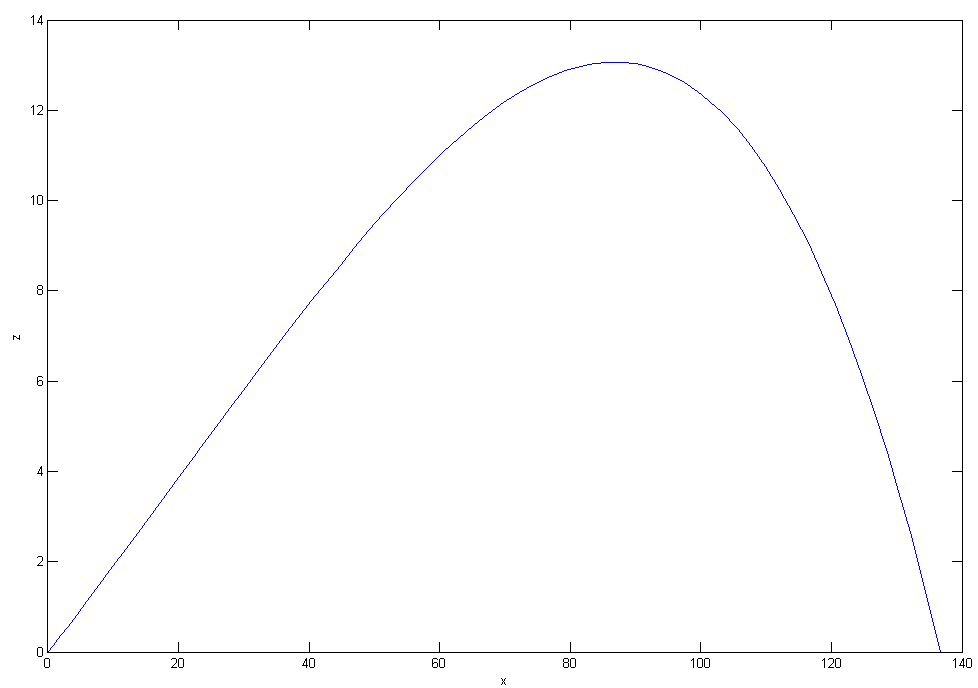
\includegraphics[scale=0.37]{../images/rr_traj_basic.png}
\caption[2D plot of an example Robinson and Robinson model trajectory]{Here we plot the distance of the
golf ball against the height, using the basic \citeauthor*{Robinson2013} model to calculate the trajectory.}
\label{2d-test-rr}
\end{figure}

In figure \ref{3d-test-rr} we display a 3 dimensional plot of the trajectory. Here we notice that 
the spin of the ball influences the movement in the $y$ plane fairly considerably, adding a deviation
from a standard projectile which we would not predict by projectile motion alone. This is the action
of the spin on the trajectory.

\begin{figure}[h]
% Also in new-golf
\centering
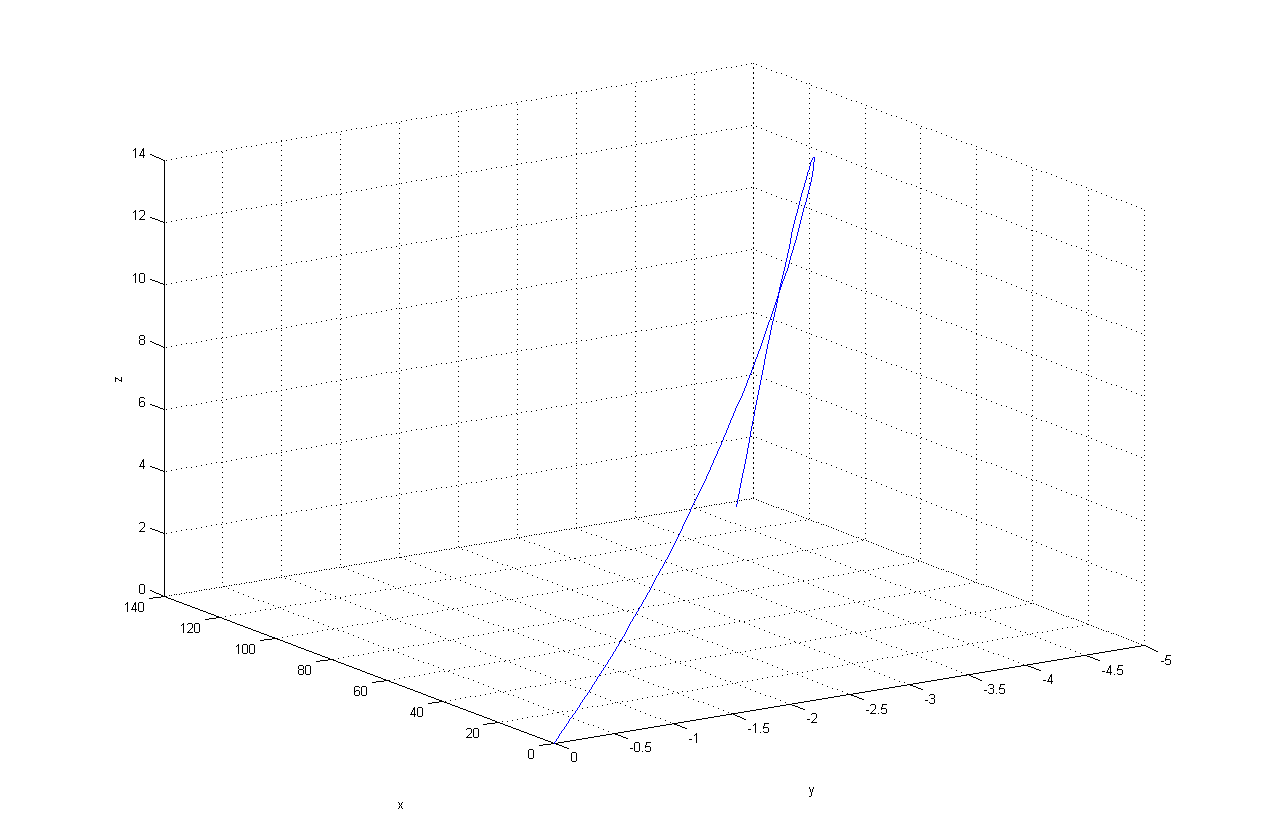
\includegraphics[scale=0.4]{../images/3d-rr.png}
\caption[3D plot of an example Robinson and Robinson model trajectory]{A 3D plot of the same model as
Figure \ref{2d-test-rr}, showing the deviation due to the spin of the ball in this model.}
\label{3d-test-rr}
\end{figure}

\pagebreak
% Describe the model, provide diagrams, show basic runs.

% Model is a good comprimise between simplicity and flexibility. Can plug in new drag coefficents.
% Some parts of the model are purely heurestic like the form for the lift, others seem just plain wrong.
% The overall structure is good though. Compare basic run to data, show similar shape but incorrect
% carry.

\section{Limitations of the Model}

While the model given by \citet{Robinson2013} is a good start, it is not without flaws. The authors
themselves admit that there are a number of points where the model could potentially be improved
\begin{itemize}
\item The model only takes into account a positive Magnus effect, but if the separation points were
to move to a different position on the ball this form would no longer apply.
\item The constant value of $c_D$ is rather troubling, particularly considering there is some experimental
evidence that the golf ball does reach the critical and supercritical domain during the course of an
average golf ball flight.
\item The form of $c_D$ and $c_L$ have no dependency on Reynolds number at all, which contradicts previous
analysis.
\item The spin of the ball is assumed constant throughout the flight. The authors state that in most
situations the loss of spin is low enough to be ignored, citing some evidence that the ball keeps a
significant proportion. This assumption is also presented in \citet{Lieberman2001}, where the simple
differential equation
\[
\dot{\omega} = -0.00002
\]
is used to model the spin decay. This constant is so small as to cause almost no change in spin over
the flight, and as such we will not concern ourselves with modelling spin decay.
\end{itemize}

The authors do state, however, that building dependency on speed and spin into their model would be
possible with the analysis they have performed, allowing these limitations to be addressed without 
drastically changing the form of the resultant equations.


The lack of any dependency on speed is addressed within \citet{Jensen2014Comment} by means of dimensional
analysis. Jensen uses a similar analysis to the previous section on drag to determine that if $c_L$ is
independent of the Reynolds number then it cannot, by dimensionality arguments, only be a function of
$\omega$. Instead, in order for the function to have some dependency on spin a possible dimensionless grouping
of $r\omega/\vv$ can be used. Jensen also suggests several other forms which $c_D$ and $c_L$ may take
based solely on dimensional considerations.

\citet{Robinson2014Reply} is the authors of \citet{Robinson2013} reply to the paper by Jensen. Robinson
and Robinson state that the second constant in \eqref{cl-rr}, as found from \citet{davies1949aerodynamics},
is given in units of $1/(\text{rad} \,\text{s}^{-1})$, and as such cancel with the units of $\omega$ and 
overall give an expression which is dimensionless, as we expect $c_L$ to be from our earlier discussion.
The authors go on to discuss the necessity and normality of having a multiplying constant which renders
an expression dimensionally consistent, giving an example based on the spring constant from Hooke's 
Law.

Robinson and Robinson also give a number of other references to experimental data confirming their
assumptions with regards to the dependency of lift on spin, and discuss some other alternative forms
of the lift force with different dependencies on the velocity of the ball.

\subsection{Comparing Trajectories with Data}

In order to improve upon the model by Robinson and Robinson

% Talk about the \citet{Jensen2014Comment} comment, dimensional analysis, lead into talking about why
% we need to improve this model to find a better form for $c_{D}$. Ppotentially a way to estimate the 
% spin ratio. Mention how \citet{Robinson2014Reply} addresses some of the concerns of the comment but does
% not give forms for $c_{D}$. Talk about how the golf ball is in the middle between the high and low
% reynold limits and this will require some matching modelling to find a good form.